\section{Introduction}

%%%%%%%%%%%%%%%%%%%%%%%%%%%%%%%%%%%%%%%%%%%%%%%%%%%%%%

\frame{\frametitle{Sanger sequencing}

aka first/former generation sequencing

\begin{columns}

	\column{0.3\textwidth}

		\begin{figure}
			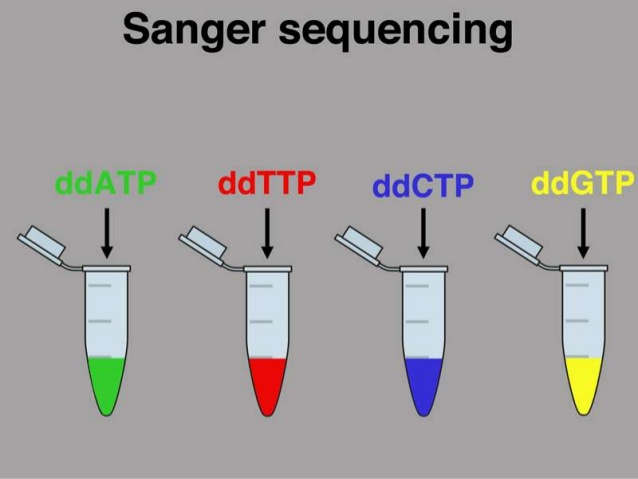
\includegraphics[scale=0.15]{Pics/sanger}
		\end{figure}

	\column{0.7\textwidth}

		\begin{figure}
			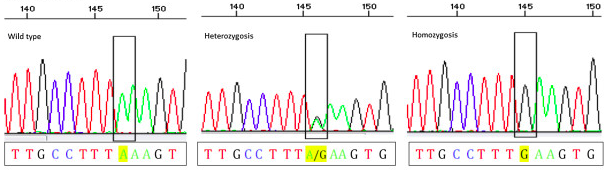
\includegraphics[scale=0.35]{Pics/sangerElectro}
		\end{figure}

\end{columns}

}

%%%%%%%%%%%%%%%%%%%%%%%%%%%%%%%%%%%%%%%%%%%%%%%%%%%%%%

\frame{\frametitle{Next Generation Sequencing}

	\begin{figure}
		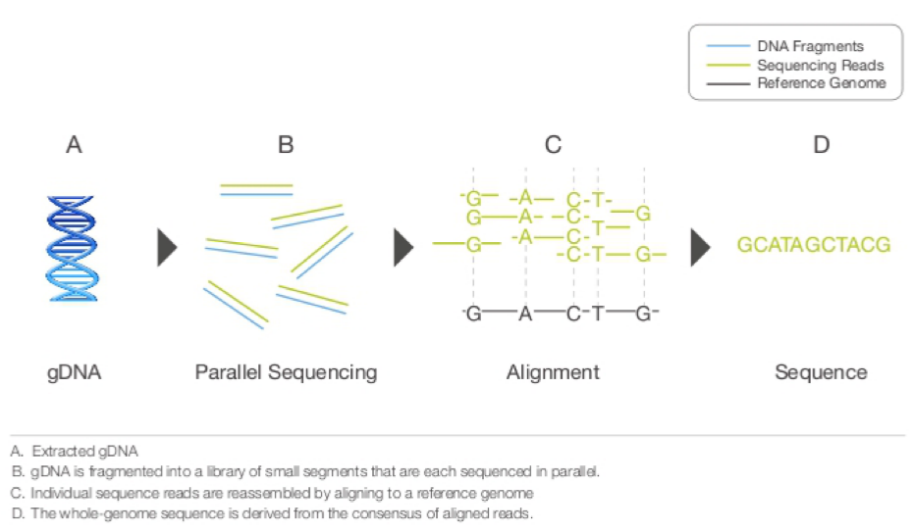
\includegraphics[scale=0.3]{Pics/illumina}
	\end{figure}

}


%%%%%%%%%%%%%%%%%%%%%%%%%%%%%%%%%%%%%%%%%%%%%%%%%%%%

\begin{frame}
\frametitle{Low-level data}

	\begin{figure}
                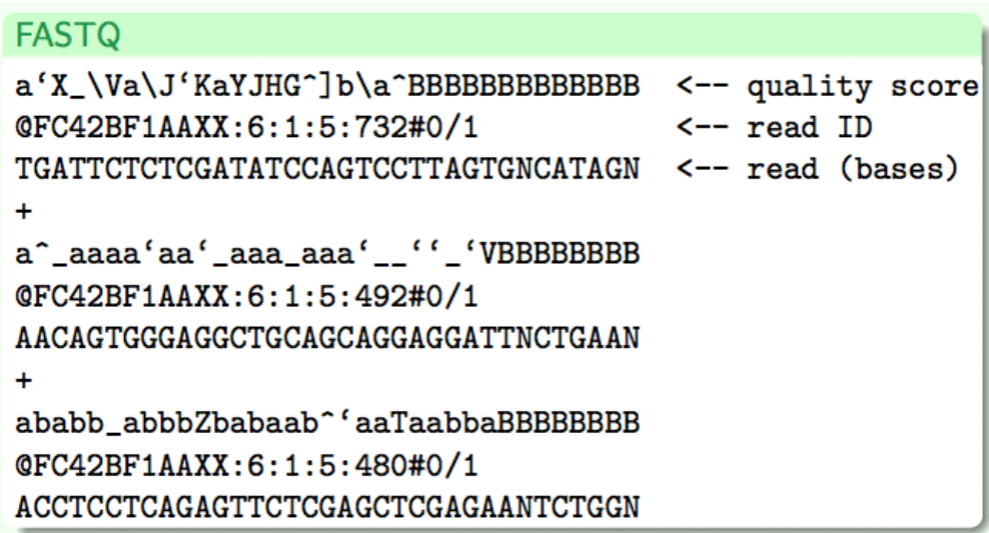
\includegraphics[width=\textwidth]{Pics/fastq.png}
        \end{figure}

\end{frame}



%%%%%%%%%%%%%%%%%%%%%%%%%%%%%%%%%%%%%%%%%%%%%%%%%%%%

\begin{frame}
\frametitle{Quality scores}

        \begin{figure}
                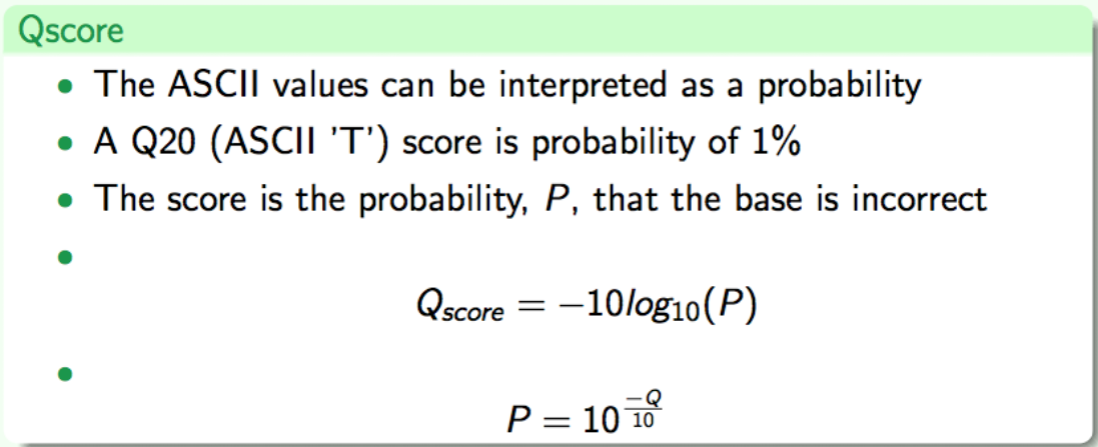
\includegraphics[width=\textwidth]{Pics/qscores.png}
        \end{figure}

\end{frame}

%%%%%%%%%%%%%%%%%%%%%%%%%%%%%%%%%%%%%%%%%%%%%%%%%%%%

\begin{frame}
\frametitle{Quality scores}

	The qscores are encoded as ASCII characters, and are shifted by +33 (now the standard) or +64.

        \begin{figure}
                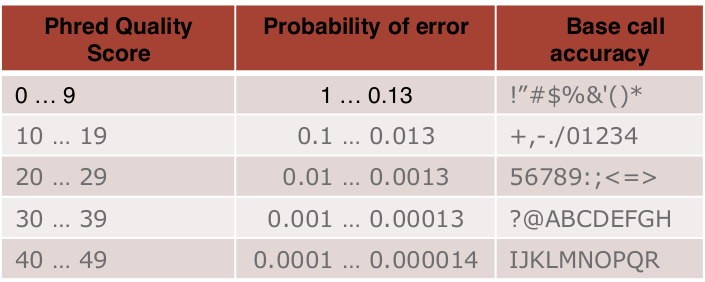
\includegraphics[width=\textwidth]{Pics/qscores_table.png}
        \end{figure}

\end{frame}

%%%%%%%%%%%%%%%%%%%%%%%%%%%%%%%%%%%%%%%%%%%%%%%%%%%%%

\begin{frame}
\frametitle{Quality scores}

	\begin{block}{Example}
		From a fastq file we observe an `A` with a qscore encoded as `7`.
		What is the probability of being `A`? What is the probability of geing `G`? 
	\end{block}

	\begin{enumerate}
		\item We find that the corresponding ASCII value of `7` is ? (hint: \url{http://www.asciitable.com})
		\pause
		\item We substract 33 to get a value of ?. This is our qscore.
		\item The probability of `A` being incorrect is ? (hint: $p=10^\frac{-Q}{10}$)
		\item The probability of `A` being correct is ?
		\item The probability of being `G` (or `C` or `T`) is ?
	\end{enumerate}

\end{frame}

%%%%%%%%%%%%%%%%%%%%%%%%%%%%%%%%%%%%%%%%%%%%%%%%%%%%%

\begin{frame}
\frametitle{FastQ files}

        \begin{figure}
                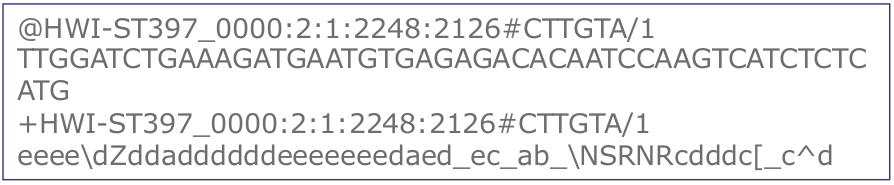
\includegraphics[width=\textwidth]{Pics/fastq_more.png}
        \end{figure}

	\begin{itemize}
		\item sequencer
		\item flowcell
		\item lane/cell/tile
		\item position within the tile
		\item barcode id for pooling/multiplexing
		\item pair
		\item ...
	\end{itemize}

\end{frame}

%%%%%%%%%%%%%%%%%%%%%%%%%%%%%%%%%%%%%%%%%%%%%%%%%%%%%

\begin{frame}
\frametitle{Quality check of fastq files: fastQC}

        \begin{figure}
                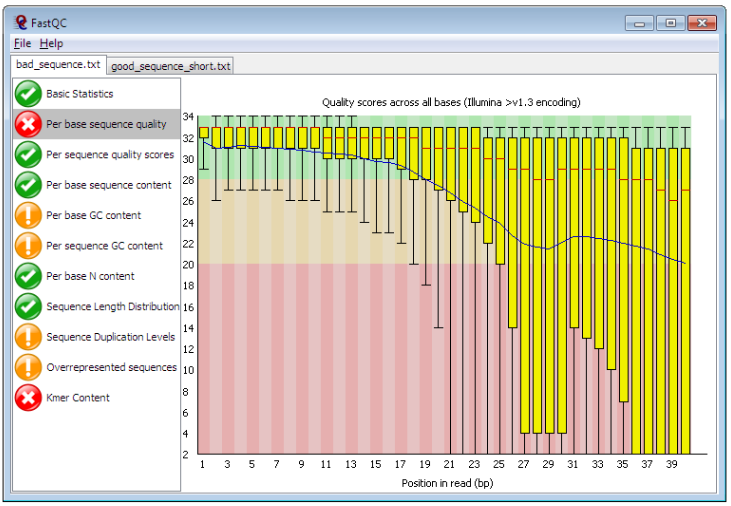
\includegraphics[width=0.7\textwidth]{Pics/fastqc.png}
        \end{figure}

	\tiny{
	\begin{itemize}
		\item distribution of qscores over read
		\item overrepresented kmers
		\item ...
	\end{itemize}
	}

	\begin{center}
		\footnotesize{\url{http://www.bioinformatics.babraham.ac.uk/projects/fastqc/}}
	\end{center}

\end{frame}

%%%%%%%%%%%%%%%%%%%%%%%%%%%%%%%%%%%%%%%%%%%%%%%%%%%%%%

\begin{frame}
\frametitle{Alignment of reads}

        \begin{figure}
                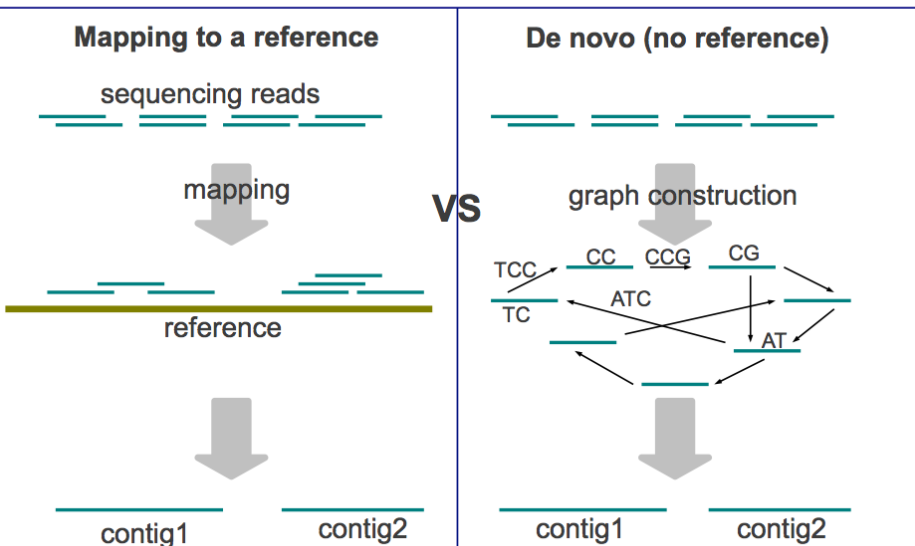
\includegraphics[width=\textwidth]{Pics/mapping.png}
        \end{figure}

\end{frame}

%%%%%%%%%%%%%%%%%%%%%%%%%%%%%%%%%%%%%%%%%%%%%%%%%%%%%

\begin{frame}
\frametitle{Mapping to a reference}

	Issues:\\
	(i) Millions of short reads.\\
	(ii) Blat/blast is too slow.\\
	But:\\
	Mate-pair gives additional information.\\

	Many aligners exists:
	\begin{itemize}
		\item Soap/soap2 (BGI)
		\item Maq/bwa (Heng Li)
		\item Bowtie/bowtie2 (Langmead B)
		\item Eland, SSAHA2,RMAP,shrimp,zoom,GEM, snap, novoAlign.
	\end{itemize}
	Most are based on burrows wheeler transform BTW (BWA,Bowtie,Soap2,...)

\end{frame}

%%%%%%%%%%%%%%%%%%%%%%%%%%%%%%%%%%%%%%%%%%%%%%%%%%%%%

\begin{frame}
\frametitle{Mapping to a reference}

	Many different aligners, what's the difference?

	\begin{itemize}
		\item Memory usage
		\item Speed
		\item Gapped (indels)
		\item Using qscores (bwa pssm)
		\item Estimating a \textbf{mappability score}
		\item Multiple best hits
		\item Paired end data
		\item Output \textbf{formats} (SAM,...)
	\end{itemize}

\end{frame}

%%%%%%%%%%%%%%%%%%%%%%%%%%%%%%%%%%%%%%%%%%%%%%%%%%%%%%

\begin{frame}
\frametitle{Alignment file}

        \begin{figure}
                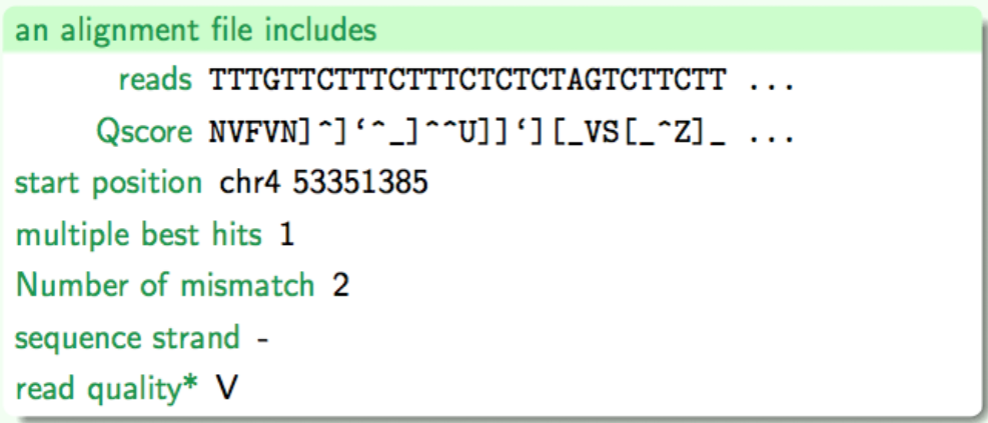
\includegraphics[width=\textwidth]{Pics/mapping_file.png}
        \end{figure}

\end{frame}


%%%%%%%%%%%%%%%%%%%%%%%%%%%%%%%%%%%%%%%%%%%%%%%%%%%%%%

\frame{\frametitle{From genomes to variants}

	\begin{figure}
		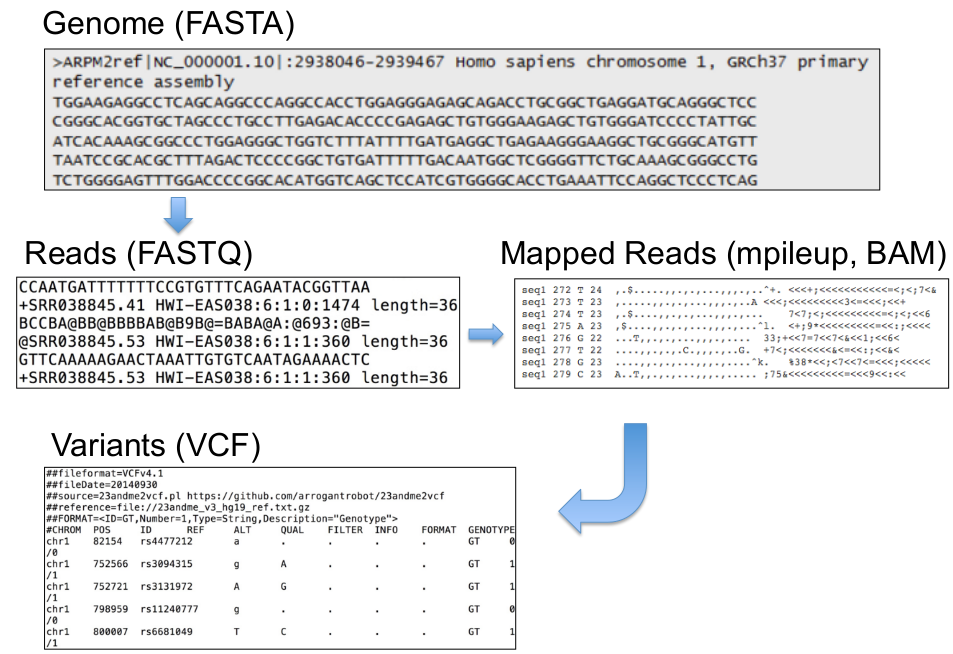
\includegraphics[width=\textwidth]{Pics/files.png}
	\end{figure}

}

%%%%%%%%%%%%%%%%%%%%%%%%%%%%%%%%%%%%%%%%%%%%%%%%

\begin{frame}
\frametitle{Our data: mapped reads with quality scores}

	\begin{figure}
                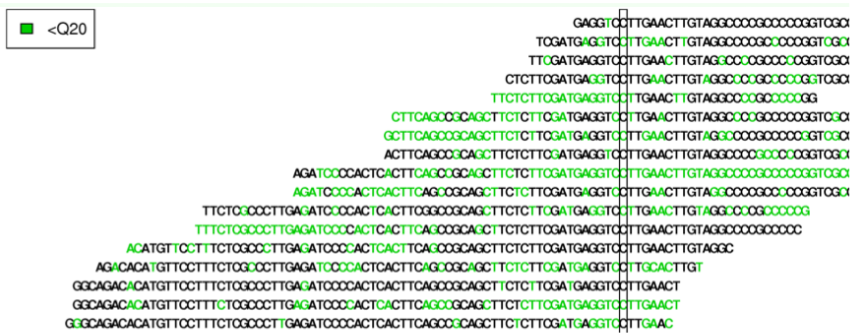
\includegraphics[width=\textwidth]{Pics/mapped_reads.png}
        \end{figure}

	\begin{itemize}
		\item Coverage:	fraction of the genome with data
		\item Depth: number of reads mapped to a position
		\item Counts: number of different alleles mapped to a position
		\item Effective Base Depth: similar to the counts, but weighing for qscores and mapping quality
	\end{itemize}

\end{frame}

%%%%%%%%%%%%%%%%%%%%%%%%%%%%%%%%%%%%%%%%%%%%%%%%%%

\frame{\frametitle{Challenges}

        \begin{figure}
                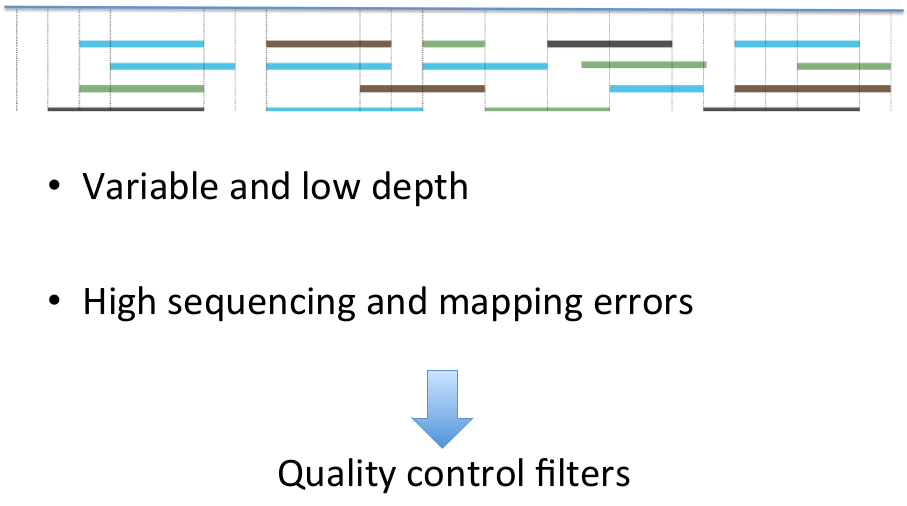
\includegraphics[width=\textwidth]{Pics/challenges.png}
        \end{figure}

}

